% Options for packages loaded elsewhere
\PassOptionsToPackage{unicode}{hyperref}
\PassOptionsToPackage{hyphens}{url}
\PassOptionsToPackage{dvipsnames,svgnames,x11names}{xcolor}
%
\documentclass[
  letterpaper,
  DIV=11,
  numbers=noendperiod]{scrreprt}

\usepackage{amsmath,amssymb}
\usepackage{iftex}
\ifPDFTeX
  \usepackage[T1]{fontenc}
  \usepackage[utf8]{inputenc}
  \usepackage{textcomp} % provide euro and other symbols
\else % if luatex or xetex
  \usepackage{unicode-math}
  \defaultfontfeatures{Scale=MatchLowercase}
  \defaultfontfeatures[\rmfamily]{Ligatures=TeX,Scale=1}
\fi
\usepackage{lmodern}
\ifPDFTeX\else  
    % xetex/luatex font selection
\fi
% Use upquote if available, for straight quotes in verbatim environments
\IfFileExists{upquote.sty}{\usepackage{upquote}}{}
\IfFileExists{microtype.sty}{% use microtype if available
  \usepackage[]{microtype}
  \UseMicrotypeSet[protrusion]{basicmath} % disable protrusion for tt fonts
}{}
\makeatletter
\@ifundefined{KOMAClassName}{% if non-KOMA class
  \IfFileExists{parskip.sty}{%
    \usepackage{parskip}
  }{% else
    \setlength{\parindent}{0pt}
    \setlength{\parskip}{6pt plus 2pt minus 1pt}}
}{% if KOMA class
  \KOMAoptions{parskip=half}}
\makeatother
\usepackage{xcolor}
\setlength{\emergencystretch}{3em} % prevent overfull lines
\setcounter{secnumdepth}{5}
% Make \paragraph and \subparagraph free-standing
\ifx\paragraph\undefined\else
  \let\oldparagraph\paragraph
  \renewcommand{\paragraph}[1]{\oldparagraph{#1}\mbox{}}
\fi
\ifx\subparagraph\undefined\else
  \let\oldsubparagraph\subparagraph
  \renewcommand{\subparagraph}[1]{\oldsubparagraph{#1}\mbox{}}
\fi


\providecommand{\tightlist}{%
  \setlength{\itemsep}{0pt}\setlength{\parskip}{0pt}}\usepackage{longtable,booktabs,array}
\usepackage{calc} % for calculating minipage widths
% Correct order of tables after \paragraph or \subparagraph
\usepackage{etoolbox}
\makeatletter
\patchcmd\longtable{\par}{\if@noskipsec\mbox{}\fi\par}{}{}
\makeatother
% Allow footnotes in longtable head/foot
\IfFileExists{footnotehyper.sty}{\usepackage{footnotehyper}}{\usepackage{footnote}}
\makesavenoteenv{longtable}
\usepackage{graphicx}
\makeatletter
\def\maxwidth{\ifdim\Gin@nat@width>\linewidth\linewidth\else\Gin@nat@width\fi}
\def\maxheight{\ifdim\Gin@nat@height>\textheight\textheight\else\Gin@nat@height\fi}
\makeatother
% Scale images if necessary, so that they will not overflow the page
% margins by default, and it is still possible to overwrite the defaults
% using explicit options in \includegraphics[width, height, ...]{}
\setkeys{Gin}{width=\maxwidth,height=\maxheight,keepaspectratio}
% Set default figure placement to htbp
\makeatletter
\def\fps@figure{htbp}
\makeatother

\KOMAoption{captions}{tableheading}
\makeatletter
\makeatother
\makeatletter
\@ifpackageloaded{bookmark}{}{\usepackage{bookmark}}
\makeatother
\makeatletter
\@ifpackageloaded{caption}{}{\usepackage{caption}}
\AtBeginDocument{%
\ifdefined\contentsname
  \renewcommand*\contentsname{Table of contents}
\else
  \newcommand\contentsname{Table of contents}
\fi
\ifdefined\listfigurename
  \renewcommand*\listfigurename{List of Figures}
\else
  \newcommand\listfigurename{List of Figures}
\fi
\ifdefined\listtablename
  \renewcommand*\listtablename{List of Tables}
\else
  \newcommand\listtablename{List of Tables}
\fi
\ifdefined\figurename
  \renewcommand*\figurename{Figure}
\else
  \newcommand\figurename{Figure}
\fi
\ifdefined\tablename
  \renewcommand*\tablename{Table}
\else
  \newcommand\tablename{Table}
\fi
}
\@ifpackageloaded{float}{}{\usepackage{float}}
\floatstyle{ruled}
\@ifundefined{c@chapter}{\newfloat{codelisting}{h}{lop}}{\newfloat{codelisting}{h}{lop}[chapter]}
\floatname{codelisting}{Listing}
\newcommand*\listoflistings{\listof{codelisting}{List of Listings}}
\makeatother
\makeatletter
\@ifpackageloaded{caption}{}{\usepackage{caption}}
\@ifpackageloaded{subcaption}{}{\usepackage{subcaption}}
\makeatother
\makeatletter
\@ifpackageloaded{tcolorbox}{}{\usepackage[skins,breakable]{tcolorbox}}
\makeatother
\makeatletter
\@ifundefined{shadecolor}{\definecolor{shadecolor}{rgb}{.97, .97, .97}}
\makeatother
\makeatletter
\makeatother
\makeatletter
\makeatother
\ifLuaTeX
  \usepackage{selnolig}  % disable illegal ligatures
\fi
\IfFileExists{bookmark.sty}{\usepackage{bookmark}}{\usepackage{hyperref}}
\IfFileExists{xurl.sty}{\usepackage{xurl}}{} % add URL line breaks if available
\urlstyle{same} % disable monospaced font for URLs
\hypersetup{
  pdftitle={Cryptography Challenge},
  pdfauthor={The Alan Turing Institute},
  colorlinks=true,
  linkcolor={blue},
  filecolor={Maroon},
  citecolor={Blue},
  urlcolor={Blue},
  pdfcreator={LaTeX via pandoc}}

\title{Cryptography Challenge}
\author{The Alan Turing Institute}
\date{2023-05-02}

\begin{document}
\maketitle
\ifdefined\Shaded\renewenvironment{Shaded}{\begin{tcolorbox}[sharp corners, enhanced, borderline west={3pt}{0pt}{shadecolor}, frame hidden, interior hidden, breakable, boxrule=0pt]}{\end{tcolorbox}}\fi

\renewcommand*\contentsname{Table of contents}
{
\hypersetup{linkcolor=}
\setcounter{tocdepth}{2}
\tableofcontents
}
\bookmarksetup{startatroot}

\hypertarget{overview}{%
\chapter*{Overview}\label{overview}}
\addcontentsline{toc}{chapter}{Overview}

\markboth{Overview}{Overview}

In this challenge, you and your team will learn about codes and ciphers:
ways of scrambling a message such that they cannot be read by unintended
people.

In the \textbf{first half of the day}, we'll be going through
\emph{symmetric ciphers}: these are ciphers where both you and the
intended recipient share the same piece of knowledge (a \emph{key}),
which is used to both encode and decode the message. In particular,
we'll spend time on \emph{substitution ciphers}, where each letter of
the alphabet is replaced with another according to some rule.

In the \textbf{second half}, we'll talk about \emph{asymmetric ciphers},
where you and the recipient do not actually share a key. Although this
might sound like a contradiction, this \emph{is} possible, and is really
important for the modern Internet, as you don't want to be sending your
key over the Internet where anybody can read it!

\bookmarksetup{startatroot}

\hypertarget{introduction-to-codes-and-ciphers}{%
\chapter{Introduction to codes and
ciphers}\label{introduction-to-codes-and-ciphers}}

\hypertarget{codes-and-ciphers}{%
\section{Codes and Ciphers}\label{codes-and-ciphers}}

We may often talk of ``code-breaking'', or the ``Enigma code'', but in
fact there is a subtle distinction between the meanings of \emph{code}
and \emph{cipher}.

A \emph{code} is a mapping from some meaningful concept (a word, or a
sentence), to an arbitrary symbol (perhaps a letter or a number). For
example, we might have a code that assigns the sentence ``It's very cold
today'' to the number ``67''. There's no particular logic behind that,
we just decided it, and wrote down this mapping in our \emph{code book}
so that it can be decoded later on.

Today though, we will be looking at \emph{ciphers}. While a \emph{code}
operates on \emph{meanings}, a \emph{cipher} operates on \emph{symbols}
(such as individual letters). It transforms the ``plaintext'' symbols to
their ``ciphertext'' counterparts using an \emph{algorithm}. This
algorithm will usually be a mathematical operation involving the
original message and some sort of \emph{key}. If someone knows (or is
able to deduce) the algorithm and the key, they will be able to decipher
an encrypted message.

\hypertarget{some-basics}{%
\section{Some basics}\label{some-basics}}

Suppose Alice wanted to send a message to her friend Bob, using a simple
``mono-alphabetic cipher'' where we replace each letter in our message
with a different letter (we'll look in more detail at this type of
cipher a bit later). The message might look like:

Tiuug Cgc,

Tgz oji lgd? Uiq'h riiq gs Rgseol!

Oupyi

\begin{quote}
\textbf{Exercise:} Could we use some simple logic and guesswork to have
a go at decrypting this? (When might Alice and Bob be planning to meet?)
\end{quote}

Hints:

\begin{itemize}
\tightlist
\item
  What are common ways of greeting people?
\item
  Since we know the names of both the sender and the recipient, could we
  look for those somewhere in the message?
\item
  Look for things like double-letters, or places where the same letter
  appears in different words.
\end{itemize}

As a very basic step, even before we worry about what encryption
algorithm to use, we can make life more difficult for someone who wants
to snoop on our messages by taking a few simple steps:

\begin{itemize}
\tightlist
\item
  Only use capital letters.
\item
  Ignore spaces, new lines, and punctuation.
\item
  Put letters into e.g.~groups of five.
\end{itemize}

It would be much harder for someone to try to decrypt:

TIUUG CGCTZ IGILG DUIQH RIIQG SRGSE OLOUP YI

than the message above!

\part{Symmetric ciphers}

As mentioned before, ciphers usually involve some sort of \emph{key},
used to encrypt and decrypt messages. Ciphers where the \emph{encryption
key} and the \emph{decryption key} are the same, are called
\emph{symmetric ciphers}. We will see a few examples here.

For symmetric ciphers, we need to worry about ``key management''. In
order for someone to read the secret message you sent them, you first
need to have shared the key - there's no point in having a sophisticated
encryption algorithm if your adversary has they key! But how do you
share it securely? (If you already have a secure communications channel
for sending the key, why do you need to encrypt your message in the
first place?)

In fact, many of the challenges in cryptography are related to designing
\emph{protocols} for ensuring that keys can be exchanged safely. The
difficulty of sharing keys is also the motivation behind the development
of \emph{asymmetric} (or public/private key) ciphers, which we'll look
at later on. For now though, we'll not worry about how we'd share keys
in practice, and we'll look at some examples of symmetric ciphers.

\hypertarget{caesar-cipher}{%
\chapter{Caesar cipher}\label{caesar-cipher}}

\hypertarget{introduction}{%
\section{Introduction}\label{introduction}}

The Caesar cipher is the most basic type of encryption that we will look
at. It is extraordinarily simple to use: each character of the alphabet
is simply mapped to another character a fixed number of alphabet away.

For example, using a shift of 2, A would be turned into C, B into D, and
so on, all the way until the end where X is turned into Z, Y back into
A, and Z into B.

You can try out the Caesar cipher with this simple form here:

Encrypt Decrypt Shift: 0 1 2 3 4 5 6 7 8 9 10 11 12 13 14 15 16 17 18 19
20 21 22 23 24 25

\hypertarget{breaking-a-caesar-cipher}{%
\section{Breaking a Caesar cipher}\label{breaking-a-caesar-cipher}}

Since there are only 25 useful possibilities for encoding, it is almost
trivial to break a Caesar cipher. You can perform a \textbf{brute-force
attack}, which means trying each possibility until you find one that
gives the correct text. For example, use the playground above to figure
out this hidden message:

\texttt{OPKKLUTLZZHNL}

\hypertarget{monoalphabetic-ciphers}{%
\chapter{Monoalphabetic ciphers}\label{monoalphabetic-ciphers}}

\hypertarget{introduction-1}{%
\section{Introduction}\label{introduction-1}}

Clearly, the Caesar cipher is not very secure. It's probably enough if
you were sending an unimaginative message to a friend, but for anything
mildly important, you probably want to crank up the security a little
bit!

The Caesar cipher is a very simple example of a \emph{monoalphabetic
substitution cipher}: one where each alphabet is replaced with another
one. This means that there's a \emph{one-to-one mapping} between pairs
of alphabet in the plain and cipher text. The problem with the Caesar
cipher is that the replacement follows a very simple pattern, so once
you know one mapping, the rest can be figured out right away.

We can go one step further and use a cipher where the mapping is
completely random. For example, A can be mapped to B, but B can be
mapped to Q, and C to I, and so on.

\begin{quote}
\textbf{Question:} How many possible encryptions are there? Would a
brute-force attack on such a cipher be sensible?
\end{quote}

Try encoding a piece of text by choosing your own cipher. You can either
enter each character of the cipher manually, or use the `randomise'
button to generate a random cipher.

\leavevmode\vadjust pre{\hypertarget{random}{}}%

\hypertarget{letters}{}
\hypertarget{a}{}
A→

\hypertarget{b}{}
B→

\hypertarget{c}{}
C→

\hypertarget{d}{}
D→

\hypertarget{e}{}
E→

\hypertarget{f}{}
F→

\hypertarget{g}{}
G→

\hypertarget{h}{}
H→

\hypertarget{i}{}
I→

\hypertarget{j}{}
J→

\hypertarget{k}{}
K→

\hypertarget{l}{}
L→

\hypertarget{m}{}
M→

\hypertarget{n}{}
N→

\hypertarget{o}{}
O→

\hypertarget{p}{}
P→

\hypertarget{q}{}
Q→

\hypertarget{r}{}
R→

\hypertarget{s}{}
S→

\hypertarget{t}{}
T→

\hypertarget{u}{}
U→

\hypertarget{v}{}
V→

\hypertarget{w}{}
W→

\hypertarget{x}{}
X→

\hypertarget{y}{}
Y→

\hypertarget{z}{}
Z→

\hypertarget{encode-remaining}{}

\hypertarget{frequency-analysis}{%
\section{Frequency analysis}\label{frequency-analysis}}

Although we realistically cannot use brute force, there is a much more
clever way to crack such a code. It relies on the fact that certain
letters of the alphabet are much more common than others in typical
English text.

Try pasting some text into the box below (or clicking the samples), and
observe the frequency distribution of the letters in the plot that
appears:

\leavevmode\vadjust pre{\hypertarget{buttons}{}}%
Samples:

\hypertarget{container}{}
\hypertarget{content}{}

\hypertarget{plot}{}

\begin{quote}
\textbf{Question:} Try a few different text sources. What are the most
and least common letters? Can you think of any reasons why this
distribution might systematically vary from text to text?

If you speak a foreign language, try analysing some text in that
language to observe how the distribution might change. (Sadly, the box
above ignores all accented characters! The schemes we're discussing
today can be adapted to work on non-English letters, but today we'll
focus only on the 26 English alphabet.)
\end{quote}

In English, the most common letter is by far `E'. If we perform the same
analysis on the cipher text, and find that `R' is the most common
letter, then it's likely that `R' decodes to `E' in the plain text.

Once we have a match, we can fill it in and try to solve the rest in an
iterative manner.

Another useful piece of information you can get from the cipher text is
to find repeated sequences of letters. For example, once you find the
letter for `E', it makes sense to look for potential spots where `THE'
might be encoded.

\hypertarget{decryption}{%
\section{Decryption}\label{decryption}}

With the above information, you should be able to have a go at
decrypting this encrypted text, with the frequency distribution shown
here:

\hypertarget{decode-container}{}
\hypertarget{content}{}

\hypertarget{decplot}{}

\leavevmode\vadjust pre{\hypertarget{check-container}{}}%

\hypertarget{decrypt_letters}{}
\hypertarget{da}{}
A→

\hypertarget{db}{}
B→

\hypertarget{dc}{}
C→

\hypertarget{dd}{}
D→

\hypertarget{de}{}
E→

\hypertarget{df}{}
F→

\hypertarget{dg}{}
G→

\hypertarget{dh}{}
H→

\hypertarget{di}{}
I→

\hypertarget{dj}{}
J→

\hypertarget{dk}{}
K→

\hypertarget{dl}{}
L→

\hypertarget{dm}{}
M→

\hypertarget{dn}{}
N→

\hypertarget{do}{}
O→

\hypertarget{dp}{}
P→

\hypertarget{dq}{}
Q→

\hypertarget{dr}{}
R→

\hypertarget{ds}{}
S→

\hypertarget{dt}{}
T→

\hypertarget{du}{}
U→

\hypertarget{dv}{}
V→

\hypertarget{dw}{}
W→

\hypertarget{dx}{}
X→

\hypertarget{dy}{}
Y→

\hypertarget{dz}{}
Z→

\hypertarget{decode-remaining}{}

\hypertarget{container}{}
\hypertarget{content}{}

\hypertarget{vigenuxe8re-cipher}{%
\chapter{Vigenère cipher}\label{vigenuxe8re-cipher}}

\hypertarget{introduction-2}{%
\section{Introduction}\label{introduction-2}}

Both the \emph{Caesar cipher} and the \emph{Monoalphabetic substitution
cipher} have a single, fixed mapping from input letters to ciphertext
letters, making them vulnerable to letter frequency analysis. It would
be more secure if we could create a \emph{polyalphabetic cipher} -
i.e.~the mapping from plaintext letters to ciphertext letters changes
after every input character. One example of this is an extension of the
Caesar cipher, called a ``Vigenère cipher'' (named after the
16th-century French diplomat Blaise de Vigenère).

In this cipher, we define the key as a word or phrase that is repeated
as many times as necessary to cover the length of the message. Each
letter in this key is then used as the key for a Caesar cipher to
encrypt the corresponding letter in the message.

For example, if the message is ``Cryptography is fun'' and the key is
``SECRETKEY'', we would write the message and the repeated key together:

\begin{verbatim}
CRYPTOGRAPHYISFUN
SECRETKEYSECRETKE
\end{verbatim}

Since the first letter of the key is ``S'', which is the 19th letter of
the alphabet, we shift the first letter of our message (``C'') by 18
(since we start counting with ``A'' as zero, meaning ``no shift''), to
give us ``U''.

\begin{quote}
\textbf{Exercise:} Using pen and paper, go ahead and encrypt the rest of
that message.
\end{quote}

\hypertarget{vig-encrypt}{}
\leavevmode\vadjust pre{\hypertarget{buttons}{}}%

\leavevmode\vadjust pre{\hypertarget{vig-answer}{}}%
UVAGXHQVYHLAZWYER

\hypertarget{cracking-the-vigenuxe8re-cipher}{%
\section{Cracking the Vigenère
cipher}\label{cracking-the-vigenuxe8re-cipher}}

Luckily, the Vigenère cipher still contains a point of weakness that we
can use to attack it: the \emph{periodicity} of the key, or in other
words, the fact that it repeats itself every \(n\) characters.

This means that, if the key length is 3, then the 1st, 4th, 7th,
\ldots{} characters are encoded in the same way, and we can tackle it
just like we did for the simple ciphers seen already.

But, to do this, we first need to know the key length!

\hypertarget{index-of-coincidence}{%
\subsection{Index of Coincidence}\label{index-of-coincidence}}

To find the key length, we need to understand another fundamental
property of English text: the \emph{index of coincidence} (IoC). If we
have a piece of text and randomly pull two letters out of it, the IoC
tells us how likely it is that these two letters are the same.

Mathematically, we can define the IoC as:

\[\text{IoC} = 26 \cdot \frac{n_\text{A}(n_\text{A} - 1) + n_\text{B}(n_\text{B} - 1) + \cdots + n_\text{Z}(n_\text{Z} - 1)}{N(N - 1)},\]

where \(n_i\) is the number of times the letter \(i\) appears in the
text, and \(N\) is the length of the text.

\begin{quote}
\textbf{Question:} Show that if all letters have the same probability of
occurring, then the IoC is equal to 1. (Assume that the text is long
enough, such that the \(n_i\)'s are much larger than 1.)
\end{quote}

Because letters are not uniformly distributed in English (recall that
'E's were particularly common), this quantity is, on average, greater
than 1 for typical English texts.

Have a play around with this plot, and find out what the IoC is for some
typical text. The same samples as before are included, plus a random
sequence of letters:

\leavevmode\vadjust pre{\hypertarget{buttons}{}}%
Samples:

\hypertarget{container}{}
\hypertarget{content}{}

\hypertarget{plot}{}

\hypertarget{using-ioc-to-determine-key-length}{%
\subsection{Using IoC to determine Key
Length}\label{using-ioc-to-determine-key-length}}

We can exploit the fact that the IoC has different values for English
text and for random sequences of letters, to identify the key length. If
the key had a length of e.g.~\textbf{4}, we would know that the 1st,
5th, 9th, \ldots{} letters were encrypted with the same letter of the
key, and we would expect the IoC of this collection of letters (and also
the 2nd, 6th, 10th, \ldots) to be higher than what we would see for
random. If on the other hand, the key had length \textbf{5}, we would
expect the same to be true if we looked at the 1st, 6th, 11th, 16th,
\ldots{} letters. (This periodic property is going to be looked at in
more detail in ``Modular Arithmetic'', which we'll cover this
afternoon.)

\begin{quote}
\textbf{Exercise:} Decrypt the following ciphertext.
\end{quote}

\hypertarget{vig-challenge}{}

\begin{quote}
\textbf{Part 1:} First, look at the Index of Coincidence and Letter
Frequency graphs for the subsets of the ciphertext that we'd expect to
see if the key length were 2, 3, or 4.
\end{quote}

Choose a key length to try:

\leavevmode\vadjust pre{\hypertarget{buttons2}{}}%
Proposed key length:

\hypertarget{vig-grid}{}
\hypertarget{vigtext-1}{}
\hypertarget{vigtext-1-text}{}

\hypertarget{vigplot-1}{}

\hypertarget{vigtext-2}{}
\hypertarget{vigtext-2-text}{}

\hypertarget{vigplot-2}{}

\hypertarget{vigtext-3}{}
\hypertarget{vigtext-3-text}{}

\hypertarget{vigplot-3}{}

\hypertarget{vigtext-4}{}
\hypertarget{vigtext-4-text}{}

\hypertarget{vigplot-4}{}

\begin{quote}
\textbf{Part 2:} Now we have identified the most likely key length, we
should be able to look at the individual letter frequency graphs, and
work out how much we'd need to shift them (like a Caesar cipher) to
identify each letter of the key.
\end{quote}

\begin{quote}
\textbf{Hint 1:} Remember, the most common letter in English text is
``E''.
\end{quote}

\begin{quote}
\textbf{Hint 2:} When we encrypt a letter using the Vigenère cipher, the
letter ``A'' corresponds to a shift of 0. So, if the most common letter
in the first of the graphs above was ``F'', this would imply that we had
a Caeser cipher of shift=1 (to move ``E''s to ``F''s), corresponding to
the first letter of the key being ``B''.
\end{quote}

Proposed Key:

\hypertarget{aside-one-time-pads---the-unbreakable-cipher}{%
\section{Aside: One-time pads - the unbreakable
cipher}\label{aside-one-time-pads---the-unbreakable-cipher}}

Since the way that we break the Vigenère cipher depends on the
repetition of the key, it follows that if the key is (at least) as long
as the message, we wouldn't be able to crack the cipher this way. In
fact, these so-called ``one-time pads'', where the key is a long
sequence of randomly generated letters, are thought to be unbreakable
(as long as the sequence is truly random, and is not re-used - hence the
name). These were used for some of the most secret communications in
World War II. However, of course, we still have the problem of how to
securely share the key between the sender and the recipient!

\hypertarget{enigma}{%
\chapter{Enigma}\label{enigma}}

\hypertarget{the-enigma-cipher-machine.}{%
\section{The Enigma cipher machine.}\label{the-enigma-cipher-machine.}}

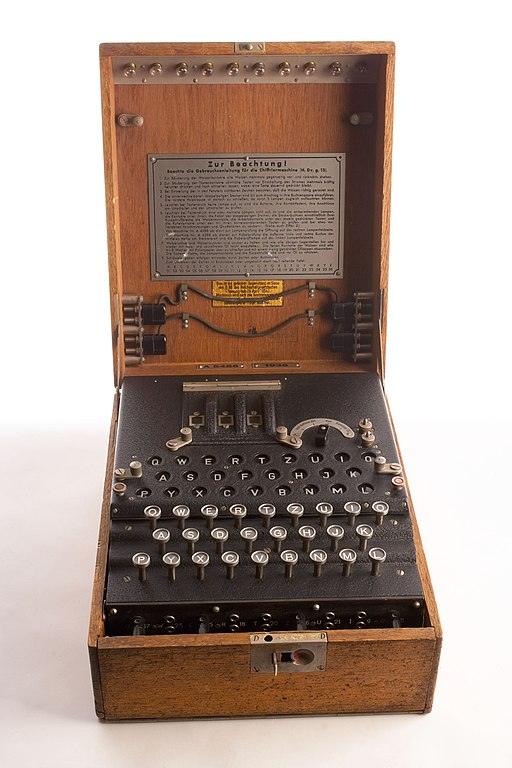
\includegraphics{images/Enigma-Machine.jpeg}

The \emph{Enigma machine} was used by the German military during World
War II to decode and encode secret communications. The simplest version
of the machine consists of:

\begin{itemize}
\tightlist
\item
  A typewriter-style keyboard, which could be used to type out the
  message.
\item
  A set of lamps, one for each letter of the alphabet. One of these
  lamps will light up every time a key on the keyboard is pressed.
\item
  Three (or later four) rotors, chosen from a selection of five, each of
  which has 26 electrical contact pins on each side, and a different
  mapping of connections between them.
\item
  An electrical \emph{reflector} next to the left-hand rotor.
\end{itemize}

The choice of which rotors to use, in which slots, and their starting
rotations, constitutes the encryption (and decryption) \emph{key}.

When the machine is setup in the specified starting position, the user
can press a key on the keyboard, and an electrical current will flow
through the rotors from right-to-left, then through the reflector, then
back through the rotors from left-to-right, and will cause a letter-lamp
to light up. At least one of the rotors will then rotate by one step
(the right-hand rotor rotates after every key press, the others less
frequently), so that when the next key is pressed, the mappings from the
keyboard to the lamps will be different.

Like Vigenère, Enigma is therefore a \emph{polyalphabetic substitution
cipher}: a given configuration of the machine is a mono-alphabetic
substitution cipher, but we get a different configuration after every
key press.

Since Enigma is a symmetric cipher, the procedure is exactly the same
for encrypting a plaintext message, or for decrypting a ciphertext
message.

\begin{quote}
\textbf{Exercise:} Have a go with the
\href{https://www.101computing.net/enigma-machine-emulator/}{Enigma
emulator}. Some things to try: - Set the starting rotors to something
(e.g.~``A,B,C''), then type out a short message. Note that after every
keypress, the right hand rotor shifts by 1. - After the end of that
message, reset the rotors to the original position, and then type out
the ciphertext that you got from the previous step. Hopefully you should
now recover the original text. - You can also try pressing the same key
many times - what do you notice about the output ciphertext?
\end{quote}

\hypertarget{cracking-the-enigma}{%
\section{Cracking the Enigma}\label{cracking-the-enigma}}

The \emph{reflector} next to the rotors gives the Enigma the nice
property that the settings for encryption and decryption are identical.
However, it also gives rise to an important flaw (which you may have
noticed from the exercise above): \emph{it is impossible for a letter to
encrypt to itself}. This means that if you have a ``crib'' (i.e.~a word
or phrase that you are fairly sure will appear in the message), and you
are trying out lots of possible keys, you can discard any where the same
letter appears in the same position in the ciphertext and the proposed
plaintext.

Using this, and various flaws in the procedures that Enigma operators
used, Polish cryptographers were able to break Enigma in the 1930s. They
then shared this knowledge with British and French cryptographers, and a
cryptographic arms race ensued that lasted throughout World War II. As
extra layers of complexity were added to Enigma (a fourth rotor, a
plug-board that mapped pairs of letters to one another, \ldots), so the
scale and complexity of the code-breaking efforts increased. An example
of this is the development of the \emph{Bombe} - an electro-mechanical
device that could try all the 17576 (26x26x26) possible rotor positions
in about 20 minutes.

\begin{figure}

{\centering 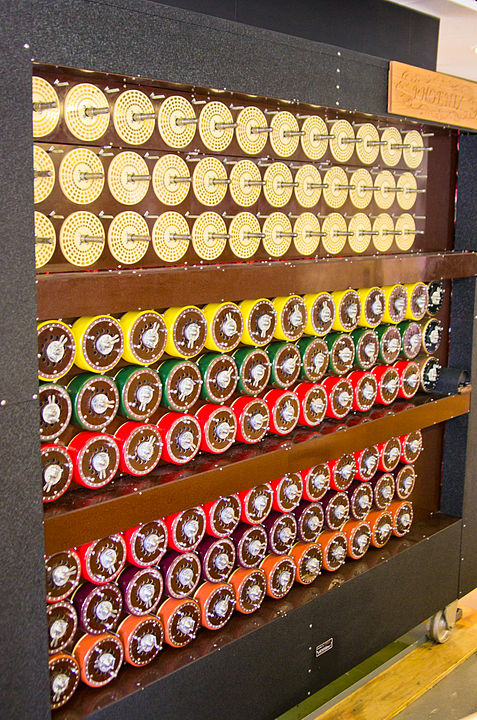
\includegraphics{images/BletchleyParkBombe.jpg}

}

\caption{The bombe at Bletchley Park. Image by Antoine Taveneaux
(license: CC-BY-SA 3.0)}

\end{figure}

\part{Asymmetric ciphers}

\emph{Asymmetric cryptography} refers to an encoding/decoding algorithm
that requires two separate keys, known as a \emph{public key} and a
\emph{private key}.

Let's say Bob wants to send Alice an encoded message that only she can
read. Alice must first generate both a public key and a private key for
herself. She sends the public key to Bob, and keeps the private key to
herself.

Bob can then use the public key to encrypt his message to Alice; and
Alice uses her private key to decrypt it. Since only Alice has the
private key, only she can decrypt the message.

You can think of this as Alice giving Bob a lock, but keeping the key
for herself.

\begin{figure}

{\centering 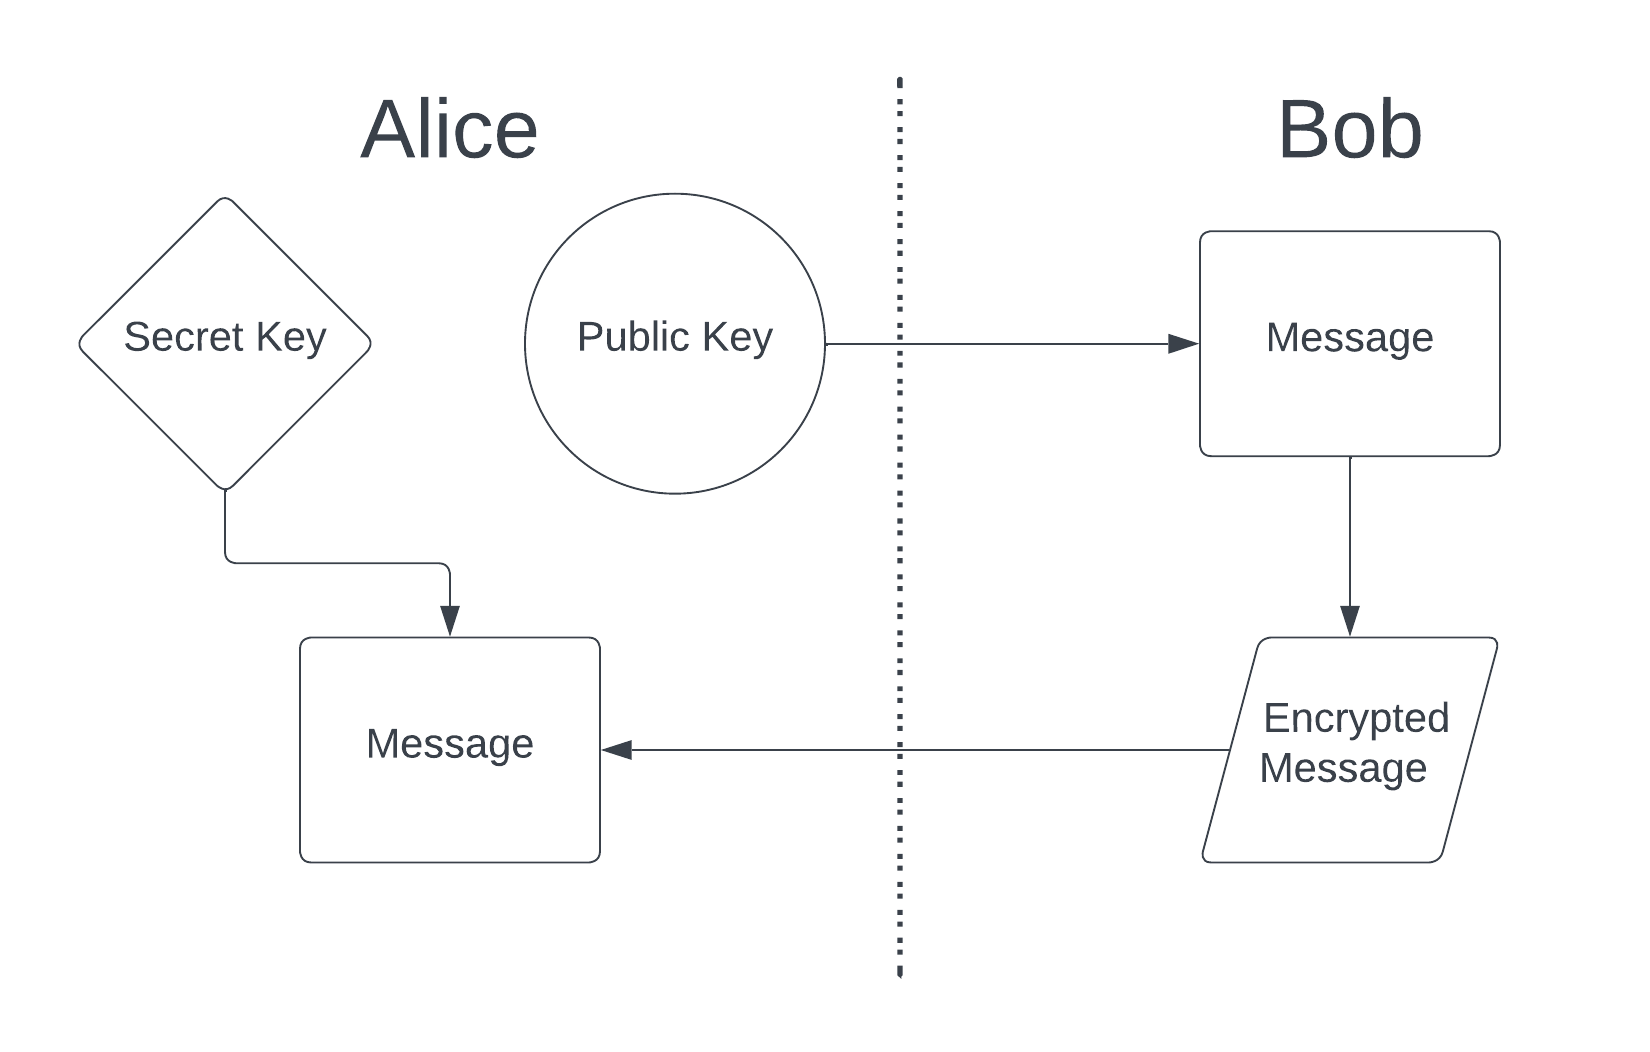
\includegraphics{images/asymmetric_public_encryption.png}

}

\caption{Alice gives Bob her public key so Bob can encrypt a message,
which she then decrypts with her private key.}

\end{figure}

In this section, we'll look at one specific example of an asymmetric
scheme, namely the RSA system.

\hypertarget{modular-arithmetic-i}{%
\chapter{Modular arithmetic I}\label{modular-arithmetic-i}}

To begin the second part of this challenge, we'll take a brief look at
\emph{modular arithmetic}. This is the same thing as regular arithmetic,
but with one twist: we only care about the remainder when dividing by
some number \(n\).

Instead of talking about numbers, we talk about numbers \emph{modulo}
\(n\). For example, \(5 \bmod 3 = 2\), because the remainder when
dividing \(5\) by \(3\) is \(2\). But also, \(8 \bmod 3 = 2\); so \(5\)
and \(8\) are equivalent, or \emph{congruent}, modulo \(3\).

Essentially, \(a\) and \(b\) are congruent modulo \(n\) if \(a\) and
\(b\) have the same remainder when divided by \(n\).

This is often denoted as:

\[5 \equiv 8 \bmod 3.\]

We can insert any other expressions we like in here, as well:

\[1 + 4 \equiv 4 \times 2 \bmod 3.\]

Another way of thinking about this is that integers `wrap around' back
to 0 after reaching \(n - 1\). So, when counting \emph{modulo} \(3\),
instead of \[0, 1, 2, 3, 4, 5, 6, 7, 8, \ldots\] we have:
\[0, 1, 2, 0, 1, 2, 0, 1, 2, \ldots\]

Because \(5\) and \(8\) both `become' the same number, they are
congruent modulo \(3\).

\begin{quote}
\textbf{Question:} Consider some other areas in life where we use
modular arithmetic without thinking about it.

What day of the week will it be, five days from now?

If you need to wake up at 7 am and you need 8 hours' sleep, what time do
you need to sleep?

Can you express these relations using modular arithmetic?
\end{quote}

\hypertarget{calculator}{%
\section{Calculator}\label{calculator}}

To help you get a feel for modular arithmetic, here is a calculator that
accepts any mathematical expression in the left-hand side. You can also
specify a modulus, and the calculator will show you the result of the
expression modulo that number. You may find this useful for the
exercises below.

\leavevmode\vadjust pre{\hypertarget{calculator}{}}%
mod

Answer: \protect\hypertarget{answer}{}{}

\hypertarget{exercises}{%
\section{Exercises}\label{exercises}}

Suppose that \(a \equiv p \bmod n\) and \(b \equiv q \bmod n\). Prove
the following statements:

\begin{enumerate}
\def\labelenumi{\arabic{enumi}.}
\tightlist
\item
  \((a + b) \equiv (p + q) \bmod n\).
\item
  \((ab) \equiv (pq) \bmod n\).
\item
  \((a^m) \equiv (p^m) \bmod n\), for all non-negative integers \(m\).
\end{enumerate}

These equalities make it far easier to perform some calculations. For
example, what is \(33^{594} \bmod{32}\)?

We might first think about calculating \(33\) to the power of \(594\),
and \emph{then} dividing that by \(32\) to find the remainder. That
sounds difficult: even a computer would struggle with such a large
number! (Try using the calculator above, or
\href{https://www.google.com/search?q=calculator}{Google's built-in
calculator}, to calculate \(33^{594}\).)

But if we notice that \(33 \equiv 1 \bmod{32}\), then we can use formula
(3) to see that

\[33^{594} \equiv 1^{594} \equiv 1 \bmod{32},\]

because \(1\) to the power of anything is still \(1\).

\begin{quote}
\textbf{Challenge:} Calculate \(7^{175} \bmod{16}\).
\end{quote}

\hypertarget{rsa-scheme-i}{%
\chapter{RSA scheme I}\label{rsa-scheme-i}}

The RSA scheme is one of the most important asymmetric-key systems, and
is widely used as part of the steps in encrypting Internet
communications.

The RSA scheme is named after the surnames of its three inventors: Ron
Rivest, Adi Shamir, and Leonard Adleman. Although they were the first to
publicly describe the RSA system in 1977, an equivalent algorithm had in
fact been discovered four years ago by Clifford Cocks, who worked at
GCHQ.

\hypertarget{introduction-3}{%
\section{Introduction}\label{introduction-3}}

The RSA scheme revolves around modular arithmetic, which the previous
page touched briefly on.

Specifically, it assumes that the message you want to transmit is first
translated into an integer \(m\) (which stands for message).

\begin{quote}
\textbf{Question:} Can you come up with a way of translating a
plain-text message into an integer?
\end{quote}

\begin{enumerate}
\def\labelenumi{\arabic{enumi}.}
\item
  The \emph{encoding} step involves the sender taking the message \(m\)
  and raising it to a power \(e\) (for `encryption'), modulo some number
  \(n\):

  \[c \equiv m^e \mod n\]

  where \(c\) is the \emph{ciphertext}. The combination of \(e\) and
  \(n\) forms the \emph{public key} of the RSA scheme.
\item
  This ciphertext is then passed to the recipient, who then
  \emph{decodes} it by raising it to a power \(d\) (for `decryption'),
  modulo \(n\):

  \[m \equiv c^d \mod n.\]

  \(d\) forms part of the \emph{private key}, which only the recipient
  is allowed to know.
\end{enumerate}

The two equations above imply together that:

\[m \equiv (m^e)^d \mod n,\]

and crucially, this is true of \emph{all} messages \(m < n\), meaning
that the keys can be used for whatever message you choose to send.

In general, if we just pick any random numbers \(e\), \(d\), and \(n\),
this will not be true! The RSA scheme works because these numbers are
specifically chosen in a way that not only satisfies the equation above,
but is also difficult to reverse-engineer.

Specifically, if you were an attacker and you knew the public key
(i.e.~\(e\) and \(n\)) \emph{as well as} the ciphertext \(c\), it's
still extremely difficult to find the correct value of \(d\) to
correctly decode the message.

\hypertarget{key-generation}{%
\section{Key generation}\label{key-generation}}

Because the RSA scheme is asymmetric, it only works for communication in
one way. The \emph{recipient} is responsible for generating the three
integers \(e\), \(d\), and \(n\). They do so using the following
algorithm:

\begin{enumerate}
\def\labelenumi{\arabic{enumi}.}
\item
  Choose two prime numbers \(p\) and \(q\), and set \(n = pq\).

  For example, if we choose \(p = 5\) and \(q = 13\), then \(n = 65\).
\item
  Calculate the \emph{totient function}, defined by
  \(\phi = (p - 1)(q - 1)\). (That symbol is the Greek letter phi.) In
  this case, we would have \(\phi = 4 \times 12 = 48\).

  Then, choose an integer \(e\) which is smaller than \(\phi\) and has
  no common prime factors with \(\phi\). Here, the only prime factors of
  \(48\) are \(2\) and \(3\): so, a valid choice would be \(e = 5\).

  \(e\) and \(n\) are part of the public key, and can be shared with the
  sender.
\item
  Finally, choose \(d\) such that \(de \equiv 1 \bmod\phi\).

  In this case, we need \(d \times 5 \equiv 1 \bmod 48\): the smallest
  value of \(d\) for which this holds true is \(d = 29\). (Can you
  verify this?)

  \(d\) is part of the private key, and must be kept secret.
\end{enumerate}

This setup ensures that regardless of what message \(m\) is being sent,
\[(m^e)^d \equiv m \bmod n,\] as required by the RSA algorithm.

Try this out using the interactive form here. It has been pre-filled
with the numbers from the example above, but you should try it out with
your own choice of numbers.

\begin{itemize}
\tightlist
\item
  \textbf{Step 1}: Choose \(p\) and \(q\) (must be prime)

  \leavevmode\vadjust pre{\hypertarget{rsa-pq-in}{}}%
  \(p\): \(q\): ~~~ ~

  \hypertarget{rsa-pq-out}{}
\item
  \textbf{Step 2}: Choose \(e\) (encryption key: must be smaller than
  \(\phi\), and cannot share prime factors with \(\phi\))

  \leavevmode\vadjust pre{\hypertarget{rsa-e-in}{}}%
  \(e\): ~~~ ~

  \hypertarget{rsa-e-out}{}
\item
  \textbf{Step 3}: Choose \(d\) (decryption key: must satisfy
  \(de \equiv 1 \bmod \phi\))

  \leavevmode\vadjust pre{\hypertarget{rsa-d-in}{}}%
  \(d\): ~~~ ~

  \hypertarget{rsa-d-out}{}
\item
  \textbf{Step 4}: Choose \(m\) (message: must be smaller than \(n\))

  \leavevmode\vadjust pre{\hypertarget{rsa-m-in}{}}%
  \(m\):

  \hypertarget{rsa-m-out}{}
\end{itemize}

\hypertarget{next-steps}{%
\section{Next steps}\label{next-steps}}

We've managed to show here that the RSA scheme \emph{works}. However,
there are several questions that remain:

\begin{enumerate}
\def\labelenumi{\arabic{enumi}.}
\tightlist
\item
  Unless you chose very small numbers for \(p\), \(q\), and \(e\), you
  probably found it hard to calculate \(d\). How can this be done
  quickly?
\item
  How do we know that the RSA scheme is \emph{secure}? Is it possible to
  obtain the private key, \(d\), if you have the public key (\(e\) and
  \(n\))?
\item
  why does the RSA algorithm work at all, i.e.~why is it always true
  that \((m^e)^d \equiv m \bmod n\)?
\end{enumerate}

We'll cover the first two questions in the remainder of today.

The proof that RSA works is provided on a bonus page, although it
doesn't form part of the activities for today, as it requires slightly
more mathematical knowledge than we've seen so far.

\hypertarget{modular-arithmetic-ii}{%
\chapter{Modular arithmetic II}\label{modular-arithmetic-ii}}

\hypertarget{introduction-4}{%
\section{Introduction}\label{introduction-4}}

In this section, we'll look at the \emph{extended Euclidean algorithm}.
An algorithm is a series of steps which can be used to solve a problem:
think of it as a recipe, but for maths.

In this case, the problem we're trying to solve is finding the values of
\(x\) and \(y\) in the equation

\[ax + by = \gcd(a, b) \tag{1}\]

where \(a\) and \(b\) are known integers, \(x\) and \(y\) are unknown
integers, and \(\gcd(a, b)\) denotes the \emph{greatest common divisor}
of \(a\) and \(b\), i.e.~the largest whole number that divides both
\(a\) and \(b\).

Formulated this way, this equation might not immediately seem relevant.
However, in fact, it is precisely what we need to find the value of
\(d\) in the RSA algorithm.

Recall that we chose \(e\) and \(d\) such that:

\begin{itemize}
\tightlist
\item
  \(e\) and \(\phi\) have no common factors. This means that
  \(\gcd(e, \phi) = 1\).
\item
  \(ed \bmod \phi = 1\).
\end{itemize}

\begin{quote}
\textbf{Question:} Reformulate the second condition in terms of equation
(1).
\end{quote}

\hypertarget{the-extended-euclidean-algorithm}{%
\section{The extended Euclidean
algorithm}\label{the-extended-euclidean-algorithm}}

You probably found above that we are trying to solve the equation
\(ed + \phi y = 1\). We already know the values of \(e\) and \(\phi\),
and the Euclidean algorithm will let us obtain the values of \(d\) and
\(y\).

Of course, we're only really interested in \(d\), so even though we'll
also get the value of \(y\), we can just throw it away.

Let's reuse the example from the previous page, where \(\phi = 48\) and
\(e = 5\). Substituting that in:

\[5d + 48y = 1\]

Each step of the Euclidean algorithm is a simple division. We start off
with the larger number (48), and divide it by the smaller number (5). In
this case, \(48\) divided by \(5\) is \(9\), with a remainder of \(3\):

\[\underset{\text{big number}}{\color{blue}{48}} = (9 \times \underset{\text{small number}}{\color{red}{5}}) + \underset{\text{remainder}}{\color{green}{3}}\]

We repeat this, but the small number from the previous equation (\(5\))
becomes the `big number', and the remainder (\(3\)) becomes the `small
number'.

\[\underset{\text{big number}}{\color{blue}{5}} = (1 \times \underset{\text{small number}}{\color{red}{3}}) + \underset{\text{remainder}}{\color{green}{2}}\]

And again:

\[\underset{\text{big number}}{\color{blue}{3}} = (1 \times \underset{\text{small number}}{\color{red}{2}}) + \underset{\text{remainder}}{\color{green}{1}}\]

We can stop when we get to the remainder of \(1\), because that's the
number on the right-hand side of our original equation!

But how does this help us to find \(d\) and \(y\)?

We can rewrite each of the equations above by bringing the remainders to
one side:

\[\begin{align}
{\color{green}{3}} &= {\color{blue}{48}} - (9 \times {\color{red}{5}}) \\
{\color{green}{2}} &= {\color{blue}{5}} - (1 \times {\color{red}{3}}) \\
{\color{green}{1}} &= {\color{blue}{3}} - (1 \times {\color{red}{2}})
\end{align}\]

At the very top, we have an equation that links 3 to our original
numbers, 48 and 5. At the bottom, we have an equation that links our
target 1 to 3 and 2. So we just need to substitute the equations above
into the ones below, in order to relate our target 1 to the original 48
and 5.

\begin{quote}
\textbf{Exercise:} Substitute the equations above into the third
equation to express 1 in terms of multiples of 48 and 5. You will have
to do this in several steps to make sure that all the 2's and 3's are
eliminated.
\end{quote}

You might eventually end up at this answer:

\[1 = (\underset{y}{2} \times \underset{\phi}{48}) + (\underset{d}{-19} \times \underset{e}{5}).\]

which suggests that \(d = -19\) and \(y = 2\).

But we can't have a negative number for \(d\)!

Thankfully, we can add and subtract multiples of \(48\) and \(5\):

\begin{align}
1 &= (2 \times 48) - (19 \times 5) \\
  &= (2 \times 48) - (5 \times 48) + (48 \times 5) - (19 \times 5) \\
  &= (\underset{y}{-3} \times \underset{\phi}{48}) + (\underset{d}{29} \times \underset{e}{5}).
\end{align}

which tells us that \(d = 29\) is a valid choice for the decryption key.

\begin{quote}
\textbf{Exercise:} Try your hand at calculating \(d\) for another set of
\(e\) and \(\phi\).

For example, if we choose \(p = 17\) and \(q = 23\), then
\(\phi = 16 \times 22 = 352\) and we can choose \(e = 13\). What is the
correct value of \(d\) for this configuration?

Your answer: \emph{d} = ~ ~~~~\protect\hypertarget{d-result}{}{}
\end{quote}

As we will soon see, the values of \(p\) and \(q\) actually used in
practice are \emph{extremely} large! It would be very unfeasible to try
and calculate \(d\) just by testing one number after another. So, having
a fast algorithm to calculate \(d\) is very important.

\hypertarget{rsa-scheme-ii}{%
\chapter{RSA scheme II}\label{rsa-scheme-ii}}

\hypertarget{security}{%
\section{Security}\label{security}}

Finally, let's explore how secure the RSA scheme really is.

Specifically, let's consider the case where as an attacker, you already
know the public key (\(n\) and \(e\)) as well as the cipher text,
\(c = m^e \bmod n\). Can you recover the message \(m\)?

\begin{quote}
\textbf{Exercise 1:} Suppose you know that \(n = 143\) and \(e = 7\).
You also know the encoded message is \(c = 41\). Can you recover the
decoded message \(m\)?

\begin{quote}
Hint: The message can be recovered using the formula
\(m = c^d \bmod n\).

Since you already know \(n\) and \(c\), the only thing you need to find
is \(d\). Recall that \(d\) is specified by the equation
\(de \equiv 1 \bmod \phi\), and \(\phi = (p - 1)(q - 1)\).

Once you have found \(d\), you can key in its value below to quickly
calculate \(m\), and submit your answer.
\end{quote}

If \emph{c} = ~, \emph{d} = , and \emph{n} = , then \emph{m} is:

Your answer: \emph{m} = ~ ~~~~\protect\hypertarget{m1-result}{}{}
\end{quote}

\begin{quote}
\textbf{Exercise 2:} Suppose you know that \(n = 373577\) and \(e = 7\).
You also know the encoded message is \(c = 226918\). Can you recover the
decoded message \(m\), using the same strategy as above?

Chances are, you can't do this on your own! However, if you're feeling
confident, you can try to guess the answer anyway:

If \emph{c} = ~, \emph{d} = , and \emph{n} = , then \emph{m} is:

Your answer: \emph{m} = ~ ~~~~\protect\hypertarget{m2-result}{}{}
\end{quote}

You probably found that the key to cracking the message is figuring out
the prime factors \(p\) and \(q\). Once you have those, you can
calculate \(\phi\) easily, and then \(d\) using the extended Euclidean
algorithm.

In the first case, this was easy enough. But in the second case, finding
\(p\) and \(q\) is a lot harder, because \(n\) is a lot bigger.

But, we could get a computer to do it!

\hypertarget{prime-factorisation}{%
\section{Prime factorisation}\label{prime-factorisation}}

Although it is pretty slow for a human to figure out the primes \(p\)
and \(q\) from their product, computers are much better at it.

Type a number into this box, and watch as the computer factorises it:

\leavevmode\vadjust pre{\hypertarget{factorise}{}}%
~~ \protect\hypertarget{factorise-result}{}{11 × 13}~~
\protect\hypertarget{factorise-time}{}{}

With this tool, you can revisit the second exercise above.

This isn't looking very promising so far, though. If the computer can
factorise \(n\) so easily, then the RSA scheme cannot be very secure at
all!

In fact, the key to getting around this is to use \textbf{\emph{really}
large numbers}: ones which even computers cannot factorise in a
reasonable amount of time.

Here are a few large numbers which you can try in the calculator above.
Notice how the time taken to factorise them increases as the numbers get
larger. You can make up your own numbers to try as well: pick a couple
of prime numbers from
\href{http://compoasso.free.fr/primelistweb/page/prime/liste_online_en.php}{this
list}, multiply them together, and see how long it takes to factorise
it.

\begin{itemize}
\tightlist
\item
  \protect\hypertarget{example1}{}{}~
\item
  \protect\hypertarget{example2}{}{}~
\item
  \protect\hypertarget{example3}{}{}~
\item
  \protect\hypertarget{example4}{}{}~
\item
  \protect\hypertarget{example5}{}{}~
\item
  \protect\hypertarget{example6}{}{}~
\item
  \protect\hypertarget{example7}{}{}~
\item
  \protect\hypertarget{example8}{}{}~
\end{itemize}

\hypertarget{rsa-in-practice}{%
\section{RSA in practice}\label{rsa-in-practice}}

Clearly, if we make \(n\) enough, there will be a point where it takes
years or even longer to factorise it.

We can't find that out for ourselves today (we don't have that much
time!), but we can make a plot of the time taken to factorise \(n\)
versus the value of \(n\). Since our values of \(n\) (as well as the
times) will span quite a wide range, we will take the base-10 logarithms
of both values when making the plot. By extrapolating the plot, we can
then figure out how large a number we would need to make RSA secure.

Start by keying in a few values of \(n\). You can use the examples above
(which have been filled in for you), or choose your own. (But make sure
that the examples are large enough that the time taken is not zero!)

Press the `factorise' button next to each value of \(n\), and the time
taken to factorise them will be displayed for you in the box next to it.
Then, when you have a few data points, click the button to plot the
graph:

\hypertarget{rsa-plot-inputs}{}
\textbf{Value of \emph{n} }

\textbf{Time (ms)}

\protect\hypertarget{plot-feedback}{}{}

\begin{quote}
\textbf{Exercise:} Using the linear regression equation (shown in the
plot title), calculate how large a value of \(n\) we need to choose in
order for our computer to take 1 year to factorise it.

(You don't need to calculate the actual value of \(n\); it will be a
very big number! Expressing it in terms of its logarithm is enough. To
give you an idea of its size, the number of digits in \(n\) is on the
order of \(\log_{10}n\).)
\end{quote}

Although that number might be enough to stop someone cracking our
messages with \emph{this computer}, it is not enough to keep out someone
using a more powerful computer and a more efficient method for
factorising numbers.

The value of \(n\) used in practical applications of the RSA algorithm
is much larger than this. It is generally recommended that \(n\) should
be at least `2048 bits' long; or in other words, it should be larger
than \(2^{2048}\)).

This is equivalent to a decimal number with about 617 digits, meaning
that \(\log_{10}n \approx 617\)!

\bookmarksetup{startatroot}

\hypertarget{cryptography-game-resources}{%
\chapter{Cryptography Game
Resources}\label{cryptography-game-resources}}

The goal of the game is to design a cryptographic protocol for
communication between your encryption and decryption teams,
communicating solely via the `public-channel'. Scoring a point for each
successfully transmitted message, and taking a point away from your
rival team for each message your hackers can decipher.

\hypertarget{asymetric-encryption-tools-rsa}{%
\section{Asymetric Encryption Tools
(RSA)}\label{asymetric-encryption-tools-rsa}}

Steps for implementing an RSA encryption scheme:

\hypertarget{key-gen-by-recipient}{%
\subsection{Key Gen (by recipient)}\label{key-gen-by-recipient}}

The goal is to compute a triple \((e, d, n=pq)\):

\begin{enumerate}
\def\labelenumi{\arabic{enumi}.}
\tightlist
\item
  Pick primes \(p, q\) such that \(n=pq > 127\), compute \(n\).
\item
  Compute totient function \(\phi=(p-1)(q-1)\) and pick \(e<\phi\) such
  that \(e\) and \(\phi\) are coprime (i.e.~\(\gcd(e, \phi)=1\)).
\item
  Pick \(d\) such that \(de \equiv 1\mod\phi\).
\item
  Send pair \((e, n)\) to sender.
\end{enumerate}

\hypertarget{encryption-and-decryption}{%
\subsection{Encryption and Decryption}\label{encryption-and-decryption}}

For a given \(n\) character long message \(s=s_0\ldots s_n\), with
characters \(\{s_i\}\), compute integer character representations
\(\{m_i\}\) using ASCII table below.

\begin{figure}

{\centering 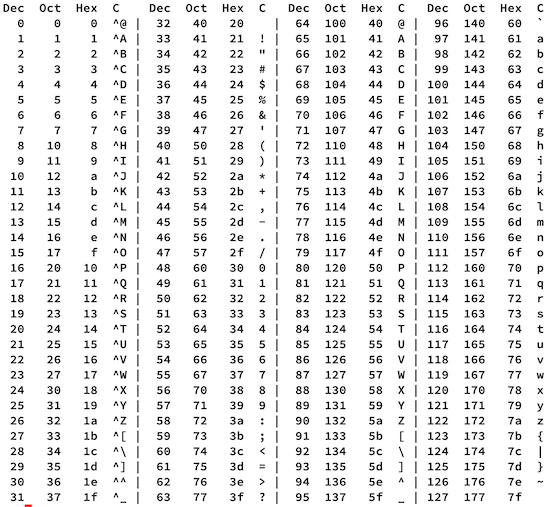
\includegraphics{images/ascii.png}

}

\caption{An ASCII character encoding table. By finding the character C
that you wish to encode the Dec encoding will give a unique integer for
that character. This can also be used to decode.}

\end{figure}

Then to encode or decode we simply need the subject, \(s\) (either a
message character integer \(m_i\), or a cipher text integer \(c_i\)),
the exponent (either \(e\) for encyption or \(d\) for decryption) and
the modulus, \(n\), to either encrypt a cipher text: \begin{equation*}
    c_i = m_i^e \mod n,
\end{equation*}

\emph{m} = ~, ~ \emph{e} = ~, ~ \emph{n} = ~ , ~ \emph{c} = ~

or decrypt a message: \begin{equation*}
    m_i = c_i^d \mod n,
\end{equation*}

\emph{c} = ~, ~ \emph{d} = ~, ~ \emph{n} = ~ , ~ \emph{m} = ~

\hypertarget{symmetric-encryption-tools}{%
\section{Symmetric Encryption Tools}\label{symmetric-encryption-tools}}

\hypertarget{ceasar-cipher}{%
\subsection{Ceasar Cipher}\label{ceasar-cipher}}

Encrypt Decrypt Shift: 0 1 2 3 4 5 6 7 8 9 10 11 12 13 14 15 16 17 18 19
20 21 22 23 24 25

\hypertarget{monoalphabetic-cipher}{%
\subsection{Monoalphabetic Cipher}\label{monoalphabetic-cipher}}

\hypertarget{encoding}{%
\subsubsection{Encoding}\label{encoding}}

Use the following tool to encode a monoalphabetic cipher text:

\leavevmode\vadjust pre{\hypertarget{random}{}}%

\hypertarget{letters}{}
\hypertarget{a}{}
A→

\hypertarget{b}{}
B→

\hypertarget{c}{}
C→

\hypertarget{d}{}
D→

\hypertarget{e}{}
E→

\hypertarget{f}{}
F→

\hypertarget{g}{}
G→

\hypertarget{h}{}
H→

\hypertarget{i}{}
I→

\hypertarget{j}{}
J→

\hypertarget{k}{}
K→

\hypertarget{l}{}
L→

\hypertarget{m}{}
M→

\hypertarget{n}{}
N→

\hypertarget{o}{}
O→

\hypertarget{p}{}
P→

\hypertarget{q}{}
Q→

\hypertarget{r}{}
R→

\hypertarget{s}{}
S→

\hypertarget{t}{}
T→

\hypertarget{u}{}
U→

\hypertarget{v}{}
V→

\hypertarget{w}{}
W→

\hypertarget{x}{}
X→

\hypertarget{y}{}
Y→

\hypertarget{z}{}
Z→

\hypertarget{encode-remaining}{}

\hypertarget{decoding}{%
\subsubsection{Decoding}\label{decoding}}

Use the following tool to decode a monoalphabetic cipher:

\hypertarget{decode-container}{}
\hypertarget{content}{}

\hypertarget{decplot}{}

\leavevmode\vadjust pre{\hypertarget{check-container}{}}%

\hypertarget{decrypt_letters}{}
\hypertarget{da}{}
A→

\hypertarget{db}{}
B→

\hypertarget{dc}{}
C→

\hypertarget{dd}{}
D→

\hypertarget{de}{}
E→

\hypertarget{df}{}
F→

\hypertarget{dg}{}
G→

\hypertarget{dh}{}
H→

\hypertarget{di}{}
I→

\hypertarget{dj}{}
J→

\hypertarget{dk}{}
K→

\hypertarget{dl}{}
L→

\hypertarget{dm}{}
M→

\hypertarget{dn}{}
N→

\hypertarget{do}{}
O→

\hypertarget{dp}{}
P→

\hypertarget{dq}{}
Q→

\hypertarget{dr}{}
R→

\hypertarget{ds}{}
S→

\hypertarget{dt}{}
T→

\hypertarget{du}{}
U→

\hypertarget{dv}{}
V→

\hypertarget{dw}{}
W→

\hypertarget{dx}{}
X→

\hypertarget{dy}{}
Y→

\hypertarget{dz}{}
Z→

\hypertarget{decode-remaining}{}

\hypertarget{container}{}
\hypertarget{content}{}

\hypertarget{vigenuxe8re-cipher-1}{%
\subsection{Vigenère Cipher}\label{vigenuxe8re-cipher-1}}

Having decided on a key use the following to encode/decode:

\hypertarget{hacking-tools}{%
\section{Hacking Tools}\label{hacking-tools}}

Here you will find collated all the tools required to break the ciphers.

\hypertarget{breaking-rsa}{%
\subsection{Breaking RSA}\label{breaking-rsa}}

To aid in cracking RSA we have provided you with a tool that computes
the quotient and remainder for two given numbers, i.e.~given numbers
\(n\) and \(d\) it returns the corresponding \(q\) and \(r\) from the
equation: \begin{equation*}
    n = q\cdot d + r
\end{equation*} HINT: This will speed up finding \(p\) and \(q\) as well
as the Euclidean algorithm!

\emph{n} = ~, ~ \emph{d} = ~, ~ \emph{q} =
~\protect\hypertarget{qh-calc}{}{}, ~ \emph{r} =
~\protect\hypertarget{rh-calc}{}{}

\hypertarget{caesar-cipher-1}{%
\subsection{Caesar Cipher}\label{caesar-cipher-1}}

Use the above tool for encoding the Caesar cipher, trying multiple
different shifts. this



\end{document}
